% Use https://www.easycalculation.com/area/polygon-centroid-point.php for centroid
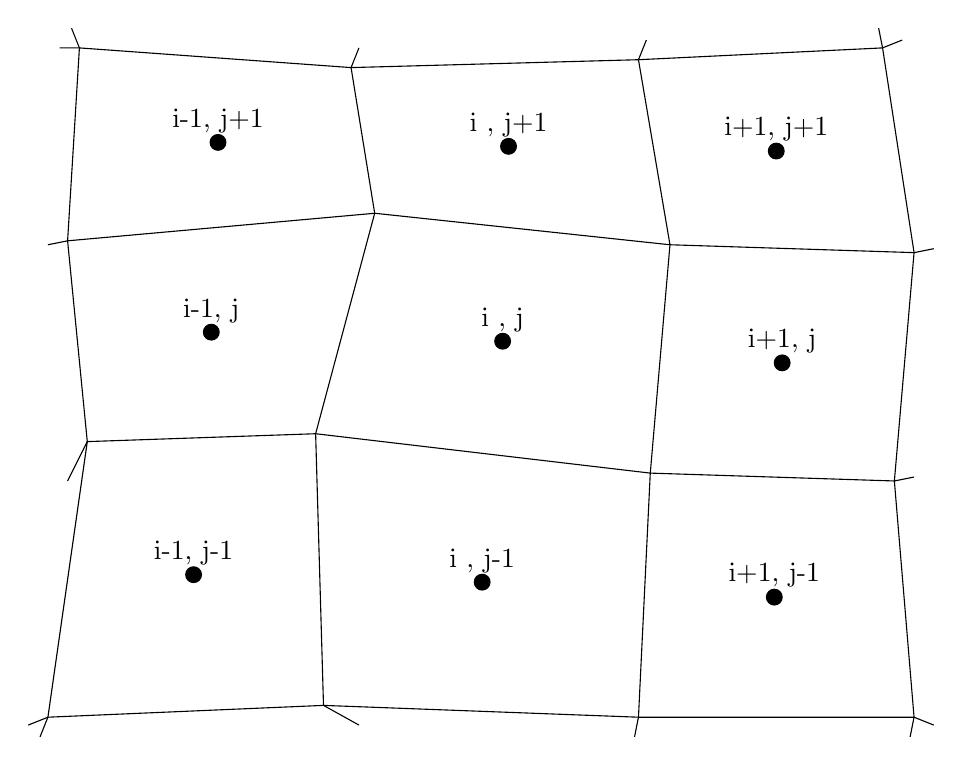
\begin{tikzpicture}[scale=5.0]
  % I lines
  \draw (-0.05,-0.02) -- (0.0,0.0) -- (0.7, 0.03) -- (1.5, 0.0) -- (2.2, 0.0) -- (2.25, -0.02);
  \draw (0.05,0.6) -- (0.1, 0.7) -- (0.68, 0.72) -- (1.53, 0.62) -- (2.15, 0.60) -- (2.2, 0.61);
  \draw (0.0, 1.2) -- (0.05, 1.21) -- (0.83, 1.28) -- (1.58, 1.2) -- (2.2, 1.18) -- (2.25, 1.19);
  \draw (0.03, 1.7) -- (0.08, 1.70) -- (0.77, 1.65) -- (1.5, 1.67) -- (2.12, 1.7) -- (2.17, 1.72);
  % J lines
  \draw (-0.02, -0.05) -- (0.0,0.0) -- (0.1, 0.7) -- (0.05, 1.21) -- (0.08, 1.70) -- (0.06, 1.75);
  \draw (0.79, -0.02) -- (0.7, 0.03) -- (0.68, 0.72) -- (0.83, 1.28) -- (0.77, 1.65) -- (0.79, 1.7);
  \draw (1.49, -0.05) -- (1.5, 0.0) -- (1.53, 0.62) -- (1.58, 1.2) -- (1.5, 1.67) -- (1.52, 1.72);
  \draw (2.19, -0.05) -- (2.2, 0.0) -- (2.15, 0.60) -- (2.2, 1.18) -- (2.12, 1.7) -- (2.11, 1.75);
  % Field points
\draw[fill] (0.370, 0.362) circle [radius=0.02] node [above] {i-1, j-1};
\draw[fill] (0.415, 0.978) circle [radius=0.02] node [above] {i-1, j    };
\draw[fill] (0.432, 1.460) circle [radius=0.02] node [above] {i-1, j+1};
\draw[fill] (1.103, 0.343) circle [radius=0.02] node [above] {i    , j-1};
\draw[fill] (1.155, 0.955) circle [radius=0.02] node [above] {i    , j    };
\draw[fill] (1.170, 1.450) circle [radius=0.02] node [above] {i    , j+1};
\draw[fill] (1.845, 0.305) circle [radius=0.02] node [above] {i+1, j-1};
\draw[fill] (1.865, 0.900) circle [radius=0.02] node [above] {i+1, j    };
\draw[fill] (1.850, 1.438) circle [radius=0.02] node [above] {i+1, j+1};
\end{tikzpicture}